\documentclass[twocolumn]{article}
\usepackage{graphicx}
\usepackage{fullpage}
\title{A brief introduction to \LaTeX document preparation system}
\author{A.T.~Hopkinson}
\date{}
\begin{document}
\maketitle

\begin{abstract}
We show some basic capabilities of the LateX system: math, figures,
references, sections...
\end{abstract}

\section{Math}
The gamma-function, denoted $\Gamma$, is usually defined via an integral,
	\begin{equation}\label{eq:integ}
\Gamma(z)=\int_0^\infty x^{z-1}e^{-x} dx \;.
	\end{equation}

\section{Numerical approximation of the gamma-function}
One of many simple approximation to the integral~(\ref{eq:integ}) is the Gergo
Nemes~\cite{gergo-nemes} formulae,
	\begin{equation}\label{eq:nemes}
\Gamma(z) \approx \sqrt{\frac{2\pi}{z} } \left(\frac{1}{e} \left(z +
\frac{1}{12z - \frac{1}{10z}}\right)\right)^z \;.
	\end{equation}

\section{Figures}
Here is an illustration of the Nemes' formula, compared to the built-in
gamma function from the standard C-library. First, figure~(\ref{fig:gpl})
shows the "latex" terminal of Gnuplot. Then, figure~(\ref{fig:pyxplot})
shows the "pdf" terminal of Pyxplot.

	\begin{figure}[h]\label{fig:gpl}
\input{fig-gpl.tex}
\caption{Nemes formula~(\ref{eq:nemes}) via gnuplot "latex" terminal.}
	\end{figure}

	\begin{figure}\label{fig:pyxplot}
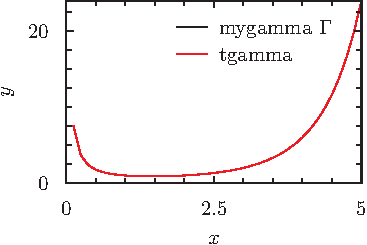
\includegraphics{fig-pyxplot.pdf}
\caption{Nemes formula~(\ref{eq:nemes}) via pyxplot "pdf" terminal.}
	\end{figure}

\begin{thebibliography}{9}
\bibitem{gergo-nemes} Nemes, Gergo (2010), "New asymptotic expansion
for the Gamma function", Archiv der Mathematik, 95 (2): 161–169,
\end{thebibliography}

\end{document}
